\documentclass[10pt]{article}
\usepackage[T1]{fontenc}
\usepackage{lmodern}
\usepackage{mathtools}
\usepackage{booktabs}
\usepackage{adjustbox}
\usepackage[left=1.5cm, right=2cm, top=1.5cm, bottom=2cm]{geometry}
\usepackage{tikz}
\usepackage{pgfplots}
\pgfplotsset{compat=1.18}
\usetikzlibrary{arrows.meta,positioning,calc}
\setlength\parindent{0pt}
\title{g7 4 - No Protection - Benchmarking Algorithm - Descending}
\date{}
\author{}

\begin{document}
\maketitle
\section*{Topology}
\begin{center}\begin{adjustbox}{max width=\linewidth}
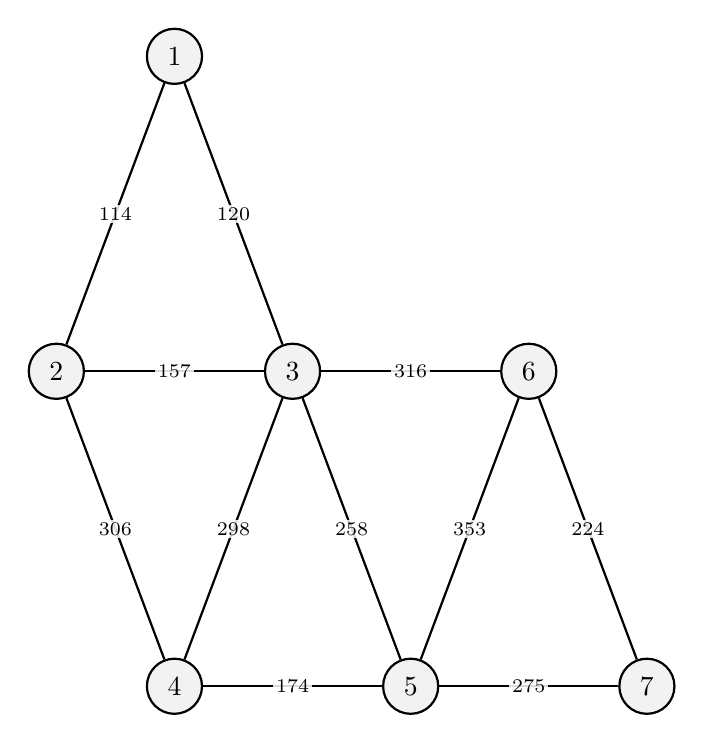
\begin{tikzpicture}[baseline, >={Stealth[length=2mm]},
  netnode/.style={circle, draw, thick, fill=gray!10, minimum size=7mm, inner sep=1pt},
  link/.style={thick},
  linklabel/.style={font=\scriptsize, inner sep=1pt, fill=white, fill opacity=0.85, text opacity=1}]
\node[netnode] (S1) at (1.500,8.000) {1};
\node[netnode] (S2) at (0.000,4.000) {2};
\node[netnode] (S3) at (3.000,4.000) {3};
\node[netnode] (S4) at (1.500,0.000) {4};
\node[netnode] (S5) at (4.500,0.000) {5};
\node[netnode] (S6) at (6.000,4.000) {6};
\node[netnode] (S7) at (7.500,0.000) {7};
\draw[link] (S1) to node[linklabel] {114} (S2);
\draw[link] (S1) to node[linklabel] {120} (S3);
\draw[link] (S2) to node[linklabel] {157} (S3);
\draw[link] (S2) to node[linklabel] {306} (S4);
\draw[link] (S3) to node[linklabel] {298} (S4);
\draw[link] (S3) to node[linklabel] {258} (S5);
\draw[link] (S3) to node[linklabel] {316} (S6);
\draw[link] (S4) to node[linklabel] {174} (S5);
\draw[link] (S5) to node[linklabel] {353} (S6);
\draw[link] (S5) to node[linklabel] {275} (S7);
\draw[link] (S6) to node[linklabel] {224} (S7);
\end{tikzpicture}
\end{adjustbox}\end{center}
\section*{Performance Parameters}
\begin{center}\begin{tabular}{lr}
\toprule
Highest link load & 749 Gb/s \\
Highest used FSU & 129 / 320 \\
Total used FSUs & 126 \\
Transponder cost & 81.5 \\
\midrule
SC-DP-QPSK transponders & 5 \\
SC-DP-16QAM transponders & 37 \\
DP-16QAM transponders & 0 \\
\bottomrule
\end{tabular}\end{center}
\clearpage
\section*{Link Load Map}
\begin{center}\begin{adjustbox}{max width=\linewidth}
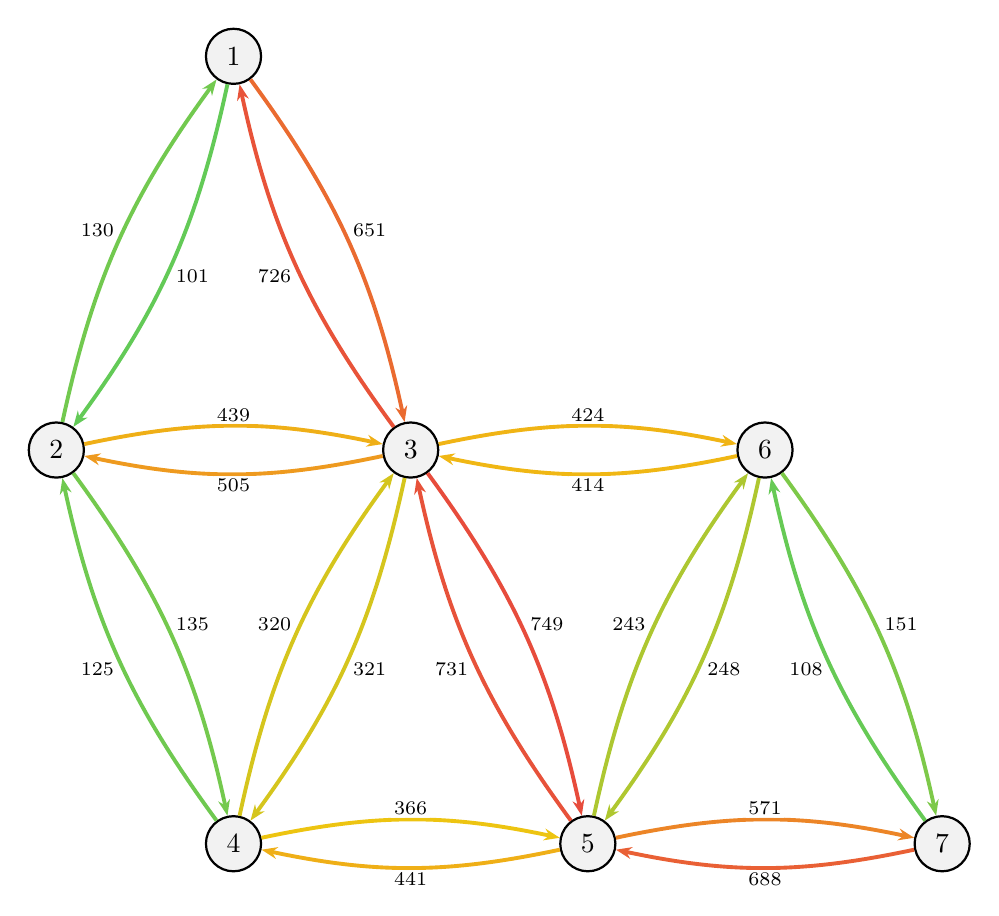
\begin{tikzpicture}[baseline, >={Stealth[length=2mm]},
  netnode/.style={circle, draw, thick, fill=gray!10, minimum size=7mm, inner sep=1pt},
  link/.style={line width=1.4pt},
  linklabel/.style={font=\scriptsize, inner sep=1pt, fill=white, fill opacity=0.85, text opacity=1}]
\node[netnode] (S1) at (2.250,10.000) {1};
\node[netnode] (S2) at (0.000,5.000) {2};
\node[netnode] (S3) at (4.500,5.000) {3};
\node[netnode] (S4) at (2.250,0.000) {4};
\node[netnode] (S5) at (6.750,0.000) {5};
\node[netnode] (S6) at (9.000,5.000) {6};
\node[netnode] (S7) at (11.250,0.000) {7};
\draw[link, ->, draw={rgb,255:red,99;green,202;blue,87}] (S1) to[bend left=12] node[linklabel, auto] {101} (S2);
\draw[link, ->, draw={rgb,255:red,234;green,107;blue,48}] (S1) to[bend left=12] node[linklabel, auto] {651} (S3);
\draw[link, ->, draw={rgb,255:red,114;green,201;blue,79}] (S2) to[bend left=12] node[linklabel, auto] {130} (S1);
\draw[link, ->, draw={rgb,255:red,239;green,175;blue,23}] (S2) to[bend left=12] node[linklabel, auto] {439} (S3);
\draw[link, ->, draw={rgb,255:red,116;green,201;blue,78}] (S2) to[bend left=12] node[linklabel, auto] {135} (S4);
\draw[link, ->, draw={rgb,255:red,232;green,83;blue,57}] (S3) to[bend left=12] node[linklabel, auto] {726} (S1);
\draw[link, ->, draw={rgb,255:red,238;green,154;blue,31}] (S3) to[bend left=12] node[linklabel, auto] {505} (S2);
\draw[link, ->, draw={rgb,255:red,213;green,197;blue,29}] (S3) to[bend left=12] node[linklabel, auto] {321} (S4);
\draw[link, ->, draw={rgb,255:red,231;green,76;blue,60}] (S3) to[bend left=12] node[linklabel, auto] {749} (S5);
\draw[link, ->, draw={rgb,255:red,240;green,180;blue,21}] (S3) to[bend left=12] node[linklabel, auto] {424} (S6);
\draw[link, ->, draw={rgb,255:red,111;green,201;blue,80}] (S4) to[bend left=12] node[linklabel, auto] {125} (S2);
\draw[link, ->, draw={rgb,255:red,213;green,197;blue,29}] (S4) to[bend left=12] node[linklabel, auto] {320} (S3);
\draw[link, ->, draw={rgb,255:red,237;green,196;blue,17}] (S4) to[bend left=12] node[linklabel, auto] {366} (S5);
\draw[link, ->, draw={rgb,255:red,231;green,82;blue,58}] (S5) to[bend left=12] node[linklabel, auto] {731} (S3);
\draw[link, ->, draw={rgb,255:red,239;green,175;blue,23}] (S5) to[bend left=12] node[linklabel, auto] {441} (S4);
\draw[link, ->, draw={rgb,255:red,173;green,199;blue,49}] (S5) to[bend left=12] node[linklabel, auto] {243} (S6);
\draw[link, ->, draw={rgb,255:red,236;green,133;blue,39}] (S5) to[bend left=12] node[linklabel, auto] {571} (S7);
\draw[link, ->, draw={rgb,255:red,240;green,183;blue,20}] (S6) to[bend left=12] node[linklabel, auto] {414} (S3);
\draw[link, ->, draw={rgb,255:red,175;green,199;blue,48}] (S6) to[bend left=12] node[linklabel, auto] {248} (S5);
\draw[link, ->, draw={rgb,255:red,125;green,201;blue,73}] (S6) to[bend left=12] node[linklabel, auto] {151} (S7);
\draw[link, ->, draw={rgb,255:red,233;green,96;blue,53}] (S7) to[bend left=12] node[linklabel, auto] {688} (S5);
\draw[link, ->, draw={rgb,255:red,102;green,202;blue,85}] (S7) to[bend left=12] node[linklabel, auto] {108} (S6);
\end{tikzpicture}
\end{adjustbox}\end{center}
\begin{center}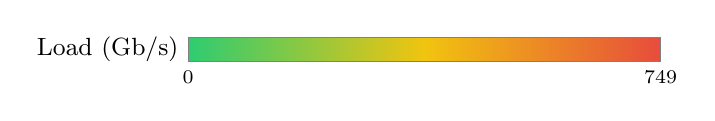
\begin{tikzpicture}
\definecolor{scalelow}{RGB}{46,204,113}\definecolor{scalemid}{RGB}{241,196,15}\definecolor{scalehigh}{RGB}{231,76,60}
\shade[left color=scalelow, right color=scalemid] (0,0) rectangle (3,0.3);
\shade[left color=scalemid, right color=scalehigh] (3,0) rectangle (6,0.3);
\draw[gray] (0,0) rectangle (6,0.3);
\node[below, font=\scriptsize] at (0,0) {0};
\node[below, font=\scriptsize] at (6,0) {749};
\node[left, font=\small] at (0,0.15) {Load (Gb/s)};
\end{tikzpicture}\end{center}
\section*{Link Load Distribution}

\begin{center}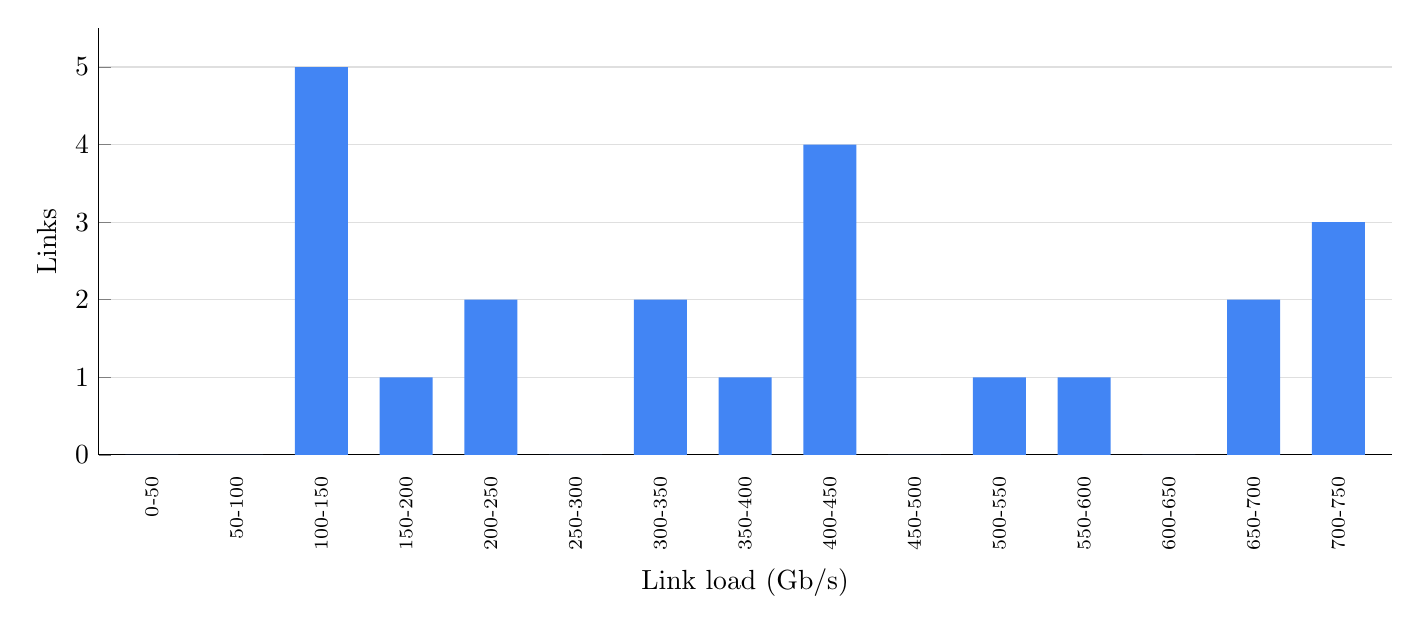
\begin{tikzpicture}
\begin{axis}[
  ybar, bar width=0.675cm, width=18.000cm, height=7cm,
  ymin=0, ymajorgrids, grid style={gray!25}, axis lines*=left,
  enlarge x limits={abs=0.675cm}, xtick=data, major x tick style={draw=none},
  x tick label style={rotate=90, font=\scriptsize, /pgf/number format/1000 sep=},
  legend style={at={(0.5,-0.3)}, anchor=north, legend columns=-1, draw=none},
  ylabel={Links},
  xlabel={Link load (Gb/s)},
  symbolic x coords={0-50,50-100,100-150,150-200,200-250,250-300,300-350,350-400,400-450,450-500,500-550,550-600,600-650,650-700,700-750}]
\addplot[fill={rgb,255:red,66;green,133;blue,244}, draw=none] coordinates {(0-50,0.000) (50-100,0.000) (100-150,5.000) (150-200,1.000) (200-250,2.000) (250-300,0.000) (300-350,2.000) (350-400,1.000) (400-450,4.000) (450-500,0.000) (500-550,1.000) (550-600,1.000) (600-650,0.000) (650-700,2.000) (700-750,3.000) };
\end{axis}
\end{tikzpicture}\end{center}
\clearpage
\section*{Spectrum Occupancy}
\begin{center}\begin{adjustbox}{max width=\linewidth}
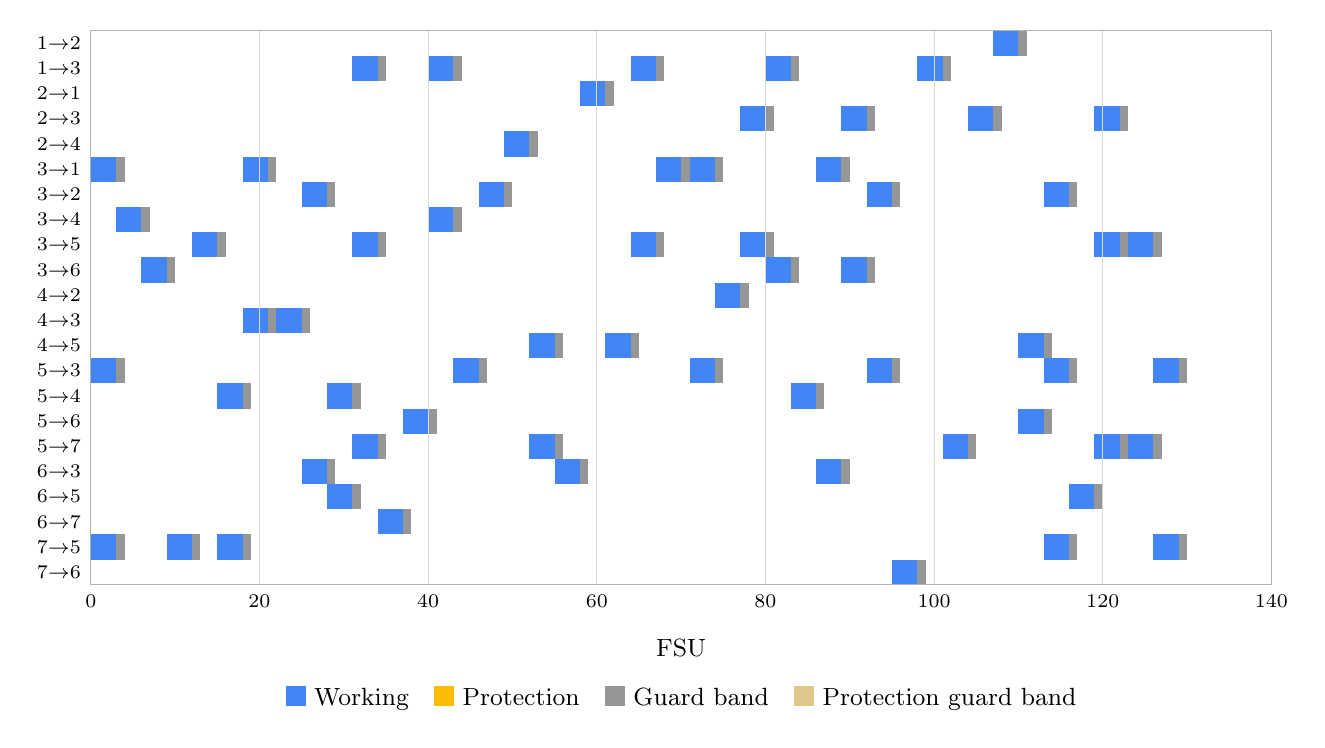
\begin{tikzpicture}[x=0.1071cm, y=-0.32cm]
\fill[fill={rgb,255:red,66;green,133;blue,244}] (107,0) rectangle (110,1);
\fill[fill={rgb,255:red,150;green,150;blue,150}] (110,0) rectangle (111,1);
\node[left, font=\scriptsize] at (0,0.5) {1\(\to\)2};
\fill[fill={rgb,255:red,66;green,133;blue,244}] (31,1) rectangle (34,2);
\fill[fill={rgb,255:red,150;green,150;blue,150}] (34,1) rectangle (35,2);
\fill[fill={rgb,255:red,66;green,133;blue,244}] (40,1) rectangle (43,2);
\fill[fill={rgb,255:red,150;green,150;blue,150}] (43,1) rectangle (44,2);
\fill[fill={rgb,255:red,66;green,133;blue,244}] (64,1) rectangle (67,2);
\fill[fill={rgb,255:red,150;green,150;blue,150}] (67,1) rectangle (68,2);
\fill[fill={rgb,255:red,66;green,133;blue,244}] (80,1) rectangle (83,2);
\fill[fill={rgb,255:red,150;green,150;blue,150}] (83,1) rectangle (84,2);
\fill[fill={rgb,255:red,66;green,133;blue,244}] (98,1) rectangle (101,2);
\fill[fill={rgb,255:red,150;green,150;blue,150}] (101,1) rectangle (102,2);
\node[left, font=\scriptsize] at (0,1.5) {1\(\to\)3};
\fill[fill={rgb,255:red,66;green,133;blue,244}] (58,2) rectangle (61,3);
\fill[fill={rgb,255:red,150;green,150;blue,150}] (61,2) rectangle (62,3);
\node[left, font=\scriptsize] at (0,2.5) {2\(\to\)1};
\fill[fill={rgb,255:red,66;green,133;blue,244}] (77,3) rectangle (80,4);
\fill[fill={rgb,255:red,150;green,150;blue,150}] (80,3) rectangle (81,4);
\fill[fill={rgb,255:red,66;green,133;blue,244}] (89,3) rectangle (92,4);
\fill[fill={rgb,255:red,150;green,150;blue,150}] (92,3) rectangle (93,4);
\fill[fill={rgb,255:red,66;green,133;blue,244}] (104,3) rectangle (107,4);
\fill[fill={rgb,255:red,150;green,150;blue,150}] (107,3) rectangle (108,4);
\fill[fill={rgb,255:red,66;green,133;blue,244}] (119,3) rectangle (122,4);
\fill[fill={rgb,255:red,150;green,150;blue,150}] (122,3) rectangle (123,4);
\node[left, font=\scriptsize] at (0,3.5) {2\(\to\)3};
\fill[fill={rgb,255:red,66;green,133;blue,244}] (49,4) rectangle (52,5);
\fill[fill={rgb,255:red,150;green,150;blue,150}] (52,4) rectangle (53,5);
\node[left, font=\scriptsize] at (0,4.5) {2\(\to\)4};
\fill[fill={rgb,255:red,66;green,133;blue,244}] (0,5) rectangle (3,6);
\fill[fill={rgb,255:red,150;green,150;blue,150}] (3,5) rectangle (4,6);
\fill[fill={rgb,255:red,66;green,133;blue,244}] (18,5) rectangle (21,6);
\fill[fill={rgb,255:red,150;green,150;blue,150}] (21,5) rectangle (22,6);
\fill[fill={rgb,255:red,66;green,133;blue,244}] (67,5) rectangle (70,6);
\fill[fill={rgb,255:red,150;green,150;blue,150}] (70,5) rectangle (71,6);
\fill[fill={rgb,255:red,66;green,133;blue,244}] (71,5) rectangle (74,6);
\fill[fill={rgb,255:red,150;green,150;blue,150}] (74,5) rectangle (75,6);
\fill[fill={rgb,255:red,66;green,133;blue,244}] (86,5) rectangle (89,6);
\fill[fill={rgb,255:red,150;green,150;blue,150}] (89,5) rectangle (90,6);
\node[left, font=\scriptsize] at (0,5.5) {3\(\to\)1};
\fill[fill={rgb,255:red,66;green,133;blue,244}] (25,6) rectangle (28,7);
\fill[fill={rgb,255:red,150;green,150;blue,150}] (28,6) rectangle (29,7);
\fill[fill={rgb,255:red,66;green,133;blue,244}] (46,6) rectangle (49,7);
\fill[fill={rgb,255:red,150;green,150;blue,150}] (49,6) rectangle (50,7);
\fill[fill={rgb,255:red,66;green,133;blue,244}] (92,6) rectangle (95,7);
\fill[fill={rgb,255:red,150;green,150;blue,150}] (95,6) rectangle (96,7);
\fill[fill={rgb,255:red,66;green,133;blue,244}] (113,6) rectangle (116,7);
\fill[fill={rgb,255:red,150;green,150;blue,150}] (116,6) rectangle (117,7);
\node[left, font=\scriptsize] at (0,6.5) {3\(\to\)2};
\fill[fill={rgb,255:red,66;green,133;blue,244}] (3,7) rectangle (6,8);
\fill[fill={rgb,255:red,150;green,150;blue,150}] (6,7) rectangle (7,8);
\fill[fill={rgb,255:red,66;green,133;blue,244}] (40,7) rectangle (43,8);
\fill[fill={rgb,255:red,150;green,150;blue,150}] (43,7) rectangle (44,8);
\node[left, font=\scriptsize] at (0,7.5) {3\(\to\)4};
\fill[fill={rgb,255:red,66;green,133;blue,244}] (12,8) rectangle (15,9);
\fill[fill={rgb,255:red,150;green,150;blue,150}] (15,8) rectangle (16,9);
\fill[fill={rgb,255:red,66;green,133;blue,244}] (31,8) rectangle (34,9);
\fill[fill={rgb,255:red,150;green,150;blue,150}] (34,8) rectangle (35,9);
\fill[fill={rgb,255:red,66;green,133;blue,244}] (64,8) rectangle (67,9);
\fill[fill={rgb,255:red,150;green,150;blue,150}] (67,8) rectangle (68,9);
\fill[fill={rgb,255:red,66;green,133;blue,244}] (77,8) rectangle (80,9);
\fill[fill={rgb,255:red,150;green,150;blue,150}] (80,8) rectangle (81,9);
\fill[fill={rgb,255:red,66;green,133;blue,244}] (119,8) rectangle (122,9);
\fill[fill={rgb,255:red,150;green,150;blue,150}] (122,8) rectangle (123,9);
\fill[fill={rgb,255:red,66;green,133;blue,244}] (123,8) rectangle (126,9);
\fill[fill={rgb,255:red,150;green,150;blue,150}] (126,8) rectangle (127,9);
\node[left, font=\scriptsize] at (0,8.5) {3\(\to\)5};
\fill[fill={rgb,255:red,66;green,133;blue,244}] (6,9) rectangle (9,10);
\fill[fill={rgb,255:red,150;green,150;blue,150}] (9,9) rectangle (10,10);
\fill[fill={rgb,255:red,66;green,133;blue,244}] (80,9) rectangle (83,10);
\fill[fill={rgb,255:red,150;green,150;blue,150}] (83,9) rectangle (84,10);
\fill[fill={rgb,255:red,66;green,133;blue,244}] (89,9) rectangle (92,10);
\fill[fill={rgb,255:red,150;green,150;blue,150}] (92,9) rectangle (93,10);
\node[left, font=\scriptsize] at (0,9.5) {3\(\to\)6};
\fill[fill={rgb,255:red,66;green,133;blue,244}] (74,10) rectangle (77,11);
\fill[fill={rgb,255:red,150;green,150;blue,150}] (77,10) rectangle (78,11);
\node[left, font=\scriptsize] at (0,10.5) {4\(\to\)2};
\fill[fill={rgb,255:red,66;green,133;blue,244}] (18,11) rectangle (21,12);
\fill[fill={rgb,255:red,150;green,150;blue,150}] (21,11) rectangle (22,12);
\fill[fill={rgb,255:red,66;green,133;blue,244}] (22,11) rectangle (25,12);
\fill[fill={rgb,255:red,150;green,150;blue,150}] (25,11) rectangle (26,12);
\node[left, font=\scriptsize] at (0,11.5) {4\(\to\)3};
\fill[fill={rgb,255:red,66;green,133;blue,244}] (52,12) rectangle (55,13);
\fill[fill={rgb,255:red,150;green,150;blue,150}] (55,12) rectangle (56,13);
\fill[fill={rgb,255:red,66;green,133;blue,244}] (61,12) rectangle (64,13);
\fill[fill={rgb,255:red,150;green,150;blue,150}] (64,12) rectangle (65,13);
\fill[fill={rgb,255:red,66;green,133;blue,244}] (110,12) rectangle (113,13);
\fill[fill={rgb,255:red,150;green,150;blue,150}] (113,12) rectangle (114,13);
\node[left, font=\scriptsize] at (0,12.5) {4\(\to\)5};
\fill[fill={rgb,255:red,66;green,133;blue,244}] (0,13) rectangle (3,14);
\fill[fill={rgb,255:red,150;green,150;blue,150}] (3,13) rectangle (4,14);
\fill[fill={rgb,255:red,66;green,133;blue,244}] (43,13) rectangle (46,14);
\fill[fill={rgb,255:red,150;green,150;blue,150}] (46,13) rectangle (47,14);
\fill[fill={rgb,255:red,66;green,133;blue,244}] (71,13) rectangle (74,14);
\fill[fill={rgb,255:red,150;green,150;blue,150}] (74,13) rectangle (75,14);
\fill[fill={rgb,255:red,66;green,133;blue,244}] (92,13) rectangle (95,14);
\fill[fill={rgb,255:red,150;green,150;blue,150}] (95,13) rectangle (96,14);
\fill[fill={rgb,255:red,66;green,133;blue,244}] (113,13) rectangle (116,14);
\fill[fill={rgb,255:red,150;green,150;blue,150}] (116,13) rectangle (117,14);
\fill[fill={rgb,255:red,66;green,133;blue,244}] (126,13) rectangle (129,14);
\fill[fill={rgb,255:red,150;green,150;blue,150}] (129,13) rectangle (130,14);
\node[left, font=\scriptsize] at (0,13.5) {5\(\to\)3};
\fill[fill={rgb,255:red,66;green,133;blue,244}] (15,14) rectangle (18,15);
\fill[fill={rgb,255:red,150;green,150;blue,150}] (18,14) rectangle (19,15);
\fill[fill={rgb,255:red,66;green,133;blue,244}] (28,14) rectangle (31,15);
\fill[fill={rgb,255:red,150;green,150;blue,150}] (31,14) rectangle (32,15);
\fill[fill={rgb,255:red,66;green,133;blue,244}] (83,14) rectangle (86,15);
\fill[fill={rgb,255:red,150;green,150;blue,150}] (86,14) rectangle (87,15);
\node[left, font=\scriptsize] at (0,14.5) {5\(\to\)4};
\fill[fill={rgb,255:red,66;green,133;blue,244}] (37,15) rectangle (40,16);
\fill[fill={rgb,255:red,150;green,150;blue,150}] (40,15) rectangle (41,16);
\fill[fill={rgb,255:red,66;green,133;blue,244}] (110,15) rectangle (113,16);
\fill[fill={rgb,255:red,150;green,150;blue,150}] (113,15) rectangle (114,16);
\node[left, font=\scriptsize] at (0,15.5) {5\(\to\)6};
\fill[fill={rgb,255:red,66;green,133;blue,244}] (31,16) rectangle (34,17);
\fill[fill={rgb,255:red,150;green,150;blue,150}] (34,16) rectangle (35,17);
\fill[fill={rgb,255:red,66;green,133;blue,244}] (52,16) rectangle (55,17);
\fill[fill={rgb,255:red,150;green,150;blue,150}] (55,16) rectangle (56,17);
\fill[fill={rgb,255:red,66;green,133;blue,244}] (101,16) rectangle (104,17);
\fill[fill={rgb,255:red,150;green,150;blue,150}] (104,16) rectangle (105,17);
\fill[fill={rgb,255:red,66;green,133;blue,244}] (119,16) rectangle (122,17);
\fill[fill={rgb,255:red,150;green,150;blue,150}] (122,16) rectangle (123,17);
\fill[fill={rgb,255:red,66;green,133;blue,244}] (123,16) rectangle (126,17);
\fill[fill={rgb,255:red,150;green,150;blue,150}] (126,16) rectangle (127,17);
\node[left, font=\scriptsize] at (0,16.5) {5\(\to\)7};
\fill[fill={rgb,255:red,66;green,133;blue,244}] (25,17) rectangle (28,18);
\fill[fill={rgb,255:red,150;green,150;blue,150}] (28,17) rectangle (29,18);
\fill[fill={rgb,255:red,66;green,133;blue,244}] (55,17) rectangle (58,18);
\fill[fill={rgb,255:red,150;green,150;blue,150}] (58,17) rectangle (59,18);
\fill[fill={rgb,255:red,66;green,133;blue,244}] (86,17) rectangle (89,18);
\fill[fill={rgb,255:red,150;green,150;blue,150}] (89,17) rectangle (90,18);
\node[left, font=\scriptsize] at (0,17.5) {6\(\to\)3};
\fill[fill={rgb,255:red,66;green,133;blue,244}] (28,18) rectangle (31,19);
\fill[fill={rgb,255:red,150;green,150;blue,150}] (31,18) rectangle (32,19);
\fill[fill={rgb,255:red,66;green,133;blue,244}] (116,18) rectangle (119,19);
\fill[fill={rgb,255:red,150;green,150;blue,150}] (119,18) rectangle (120,19);
\node[left, font=\scriptsize] at (0,18.5) {6\(\to\)5};
\fill[fill={rgb,255:red,66;green,133;blue,244}] (34,19) rectangle (37,20);
\fill[fill={rgb,255:red,150;green,150;blue,150}] (37,19) rectangle (38,20);
\node[left, font=\scriptsize] at (0,19.5) {6\(\to\)7};
\fill[fill={rgb,255:red,66;green,133;blue,244}] (0,20) rectangle (3,21);
\fill[fill={rgb,255:red,150;green,150;blue,150}] (3,20) rectangle (4,21);
\fill[fill={rgb,255:red,66;green,133;blue,244}] (9,20) rectangle (12,21);
\fill[fill={rgb,255:red,150;green,150;blue,150}] (12,20) rectangle (13,21);
\fill[fill={rgb,255:red,66;green,133;blue,244}] (15,20) rectangle (18,21);
\fill[fill={rgb,255:red,150;green,150;blue,150}] (18,20) rectangle (19,21);
\fill[fill={rgb,255:red,66;green,133;blue,244}] (113,20) rectangle (116,21);
\fill[fill={rgb,255:red,150;green,150;blue,150}] (116,20) rectangle (117,21);
\fill[fill={rgb,255:red,66;green,133;blue,244}] (126,20) rectangle (129,21);
\fill[fill={rgb,255:red,150;green,150;blue,150}] (129,20) rectangle (130,21);
\node[left, font=\scriptsize] at (0,20.5) {7\(\to\)5};
\fill[fill={rgb,255:red,66;green,133;blue,244}] (95,21) rectangle (98,22);
\fill[fill={rgb,255:red,150;green,150;blue,150}] (98,21) rectangle (99,22);
\node[left, font=\scriptsize] at (0,21.5) {7\(\to\)6};
\foreach \s in {0,20,...,140} {\draw[gray!30] (\s,0) -- (\s,22); \node[below, font=\scriptsize] at (\s,22) {\s};}
\draw[gray!60] (0,0) rectangle (140,22);
\node[font=\small] at (70.0,24.5) {FSU};
\node[font=\small] at (70.0,26.5) {\textcolor[RGB]{66,133,244}{\rule{2.5mm}{2.5mm}} Working\quad \textcolor[RGB]{251,188,5}{\rule{2.5mm}{2.5mm}} Protection\quad \textcolor[RGB]{150,150,150}{\rule{2.5mm}{2.5mm}} Guard band\quad \textcolor[RGB]{222,200,140}{\rule{2.5mm}{2.5mm}} Protection guard band\quad };
\end{tikzpicture}
\end{adjustbox}\end{center}
\clearpage
\section*{Path Length Distribution}

\begin{center}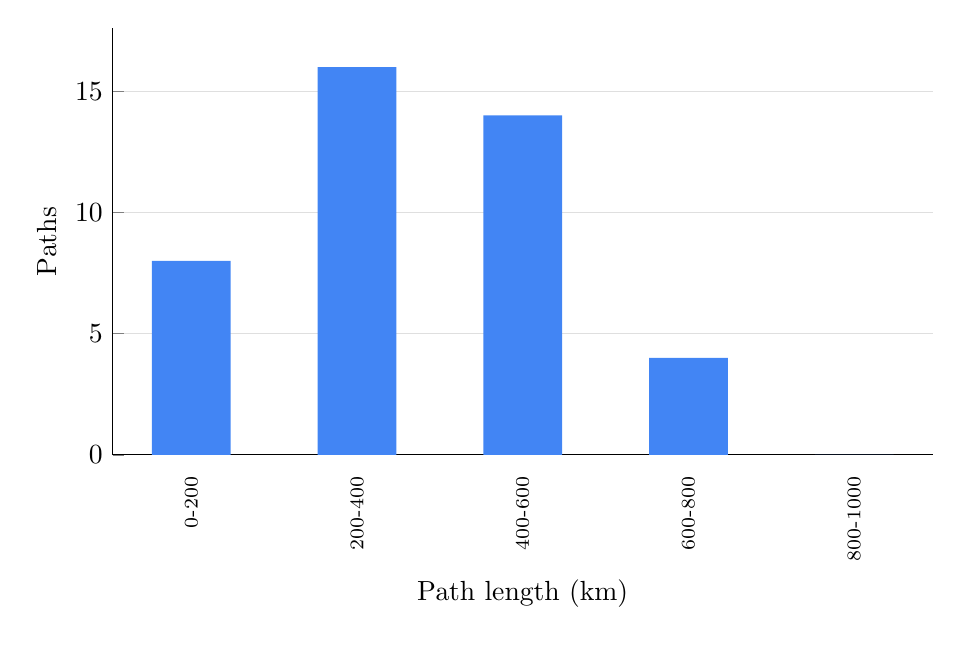
\begin{tikzpicture}
\begin{axis}[
  ybar, bar width=1.000cm, width=12.000cm, height=7cm,
  ymin=0, ymajorgrids, grid style={gray!25}, axis lines*=left,
  enlarge x limits={abs=1.000cm}, xtick=data, major x tick style={draw=none},
  x tick label style={rotate=90, font=\scriptsize, /pgf/number format/1000 sep=},
  legend style={at={(0.5,-0.3)}, anchor=north, legend columns=-1, draw=none},
  ylabel={Paths},
  xlabel={Path length (km)},
  symbolic x coords={0-200,200-400,400-600,600-800,800-1000,1000-1200,1200-1400,1400-1600,1600-1800,1800-2000}]
\addplot[fill={rgb,255:red,66;green,133;blue,244}, draw=none] coordinates {(0-200,8.000) (200-400,16.000) (400-600,14.000) (600-800,4.000) (800-1000,0.000) };
\end{axis}
\end{tikzpicture}\end{center}
\clearpage
\section*{Utilization Entropy}
\begin{center}\begin{adjustbox}{max width=\linewidth}
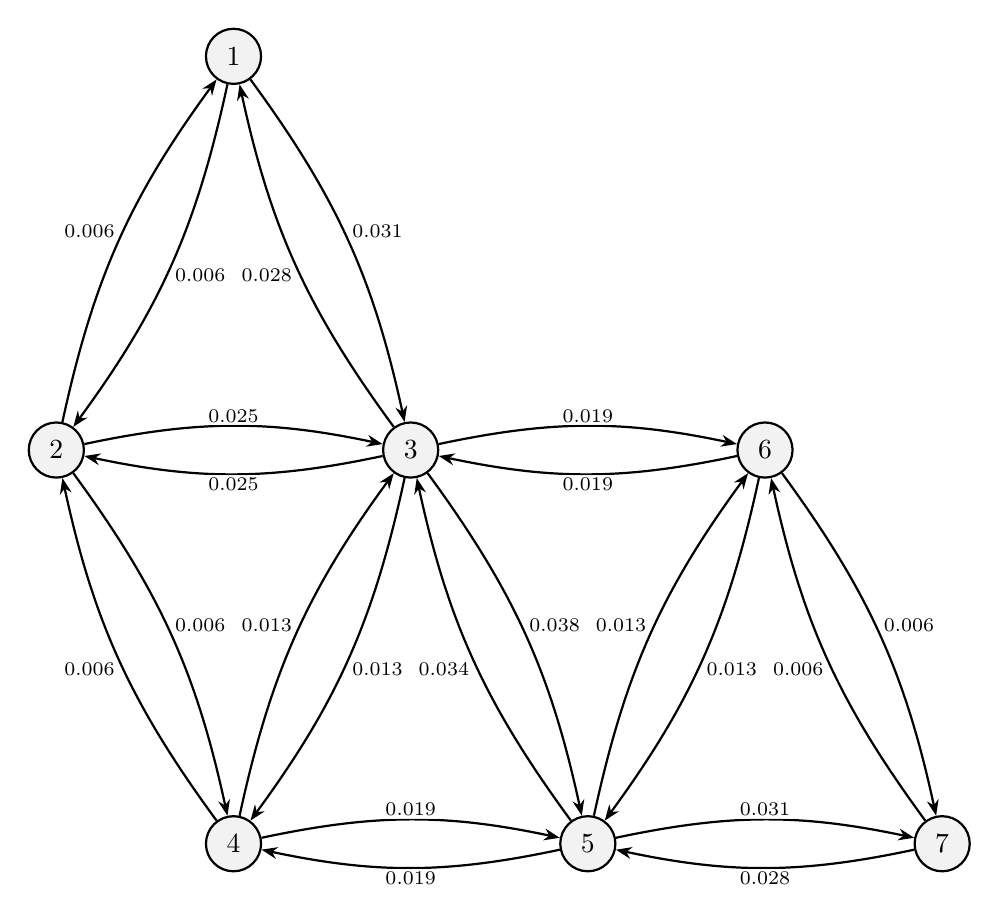
\begin{tikzpicture}[baseline, >={Stealth[length=2mm]},
  netnode/.style={circle, draw, thick, fill=gray!10, minimum size=7mm, inner sep=1pt},
  link/.style={thick},
  linklabel/.style={font=\scriptsize, inner sep=1pt, fill=white, fill opacity=0.85, text opacity=1}]
\node[netnode] (S1) at (2.250,10.000) {1};
\node[netnode] (S2) at (0.000,5.000) {2};
\node[netnode] (S3) at (4.500,5.000) {3};
\node[netnode] (S4) at (2.250,0.000) {4};
\node[netnode] (S5) at (6.750,0.000) {5};
\node[netnode] (S6) at (9.000,5.000) {6};
\node[netnode] (S7) at (11.250,0.000) {7};
\draw[link, ->] (S1) to[bend left=12] node[linklabel, auto] {0.006} (S2);
\draw[link, ->] (S1) to[bend left=12] node[linklabel, auto] {0.031} (S3);
\draw[link, ->] (S2) to[bend left=12] node[linklabel, auto] {0.006} (S1);
\draw[link, ->] (S2) to[bend left=12] node[linklabel, auto] {0.025} (S3);
\draw[link, ->] (S2) to[bend left=12] node[linklabel, auto] {0.006} (S4);
\draw[link, ->] (S3) to[bend left=12] node[linklabel, auto] {0.028} (S1);
\draw[link, ->] (S3) to[bend left=12] node[linklabel, auto] {0.025} (S2);
\draw[link, ->] (S3) to[bend left=12] node[linklabel, auto] {0.013} (S4);
\draw[link, ->] (S3) to[bend left=12] node[linklabel, auto] {0.038} (S5);
\draw[link, ->] (S3) to[bend left=12] node[linklabel, auto] {0.019} (S6);
\draw[link, ->] (S4) to[bend left=12] node[linklabel, auto] {0.006} (S2);
\draw[link, ->] (S4) to[bend left=12] node[linklabel, auto] {0.013} (S3);
\draw[link, ->] (S4) to[bend left=12] node[linklabel, auto] {0.019} (S5);
\draw[link, ->] (S5) to[bend left=12] node[linklabel, auto] {0.034} (S3);
\draw[link, ->] (S5) to[bend left=12] node[linklabel, auto] {0.019} (S4);
\draw[link, ->] (S5) to[bend left=12] node[linklabel, auto] {0.013} (S6);
\draw[link, ->] (S5) to[bend left=12] node[linklabel, auto] {0.031} (S7);
\draw[link, ->] (S6) to[bend left=12] node[linklabel, auto] {0.019} (S3);
\draw[link, ->] (S6) to[bend left=12] node[linklabel, auto] {0.013} (S5);
\draw[link, ->] (S6) to[bend left=12] node[linklabel, auto] {0.006} (S7);
\draw[link, ->] (S7) to[bend left=12] node[linklabel, auto] {0.028} (S5);
\draw[link, ->] (S7) to[bend left=12] node[linklabel, auto] {0.006} (S6);
\end{tikzpicture}
\end{adjustbox}\end{center}

\begin{center}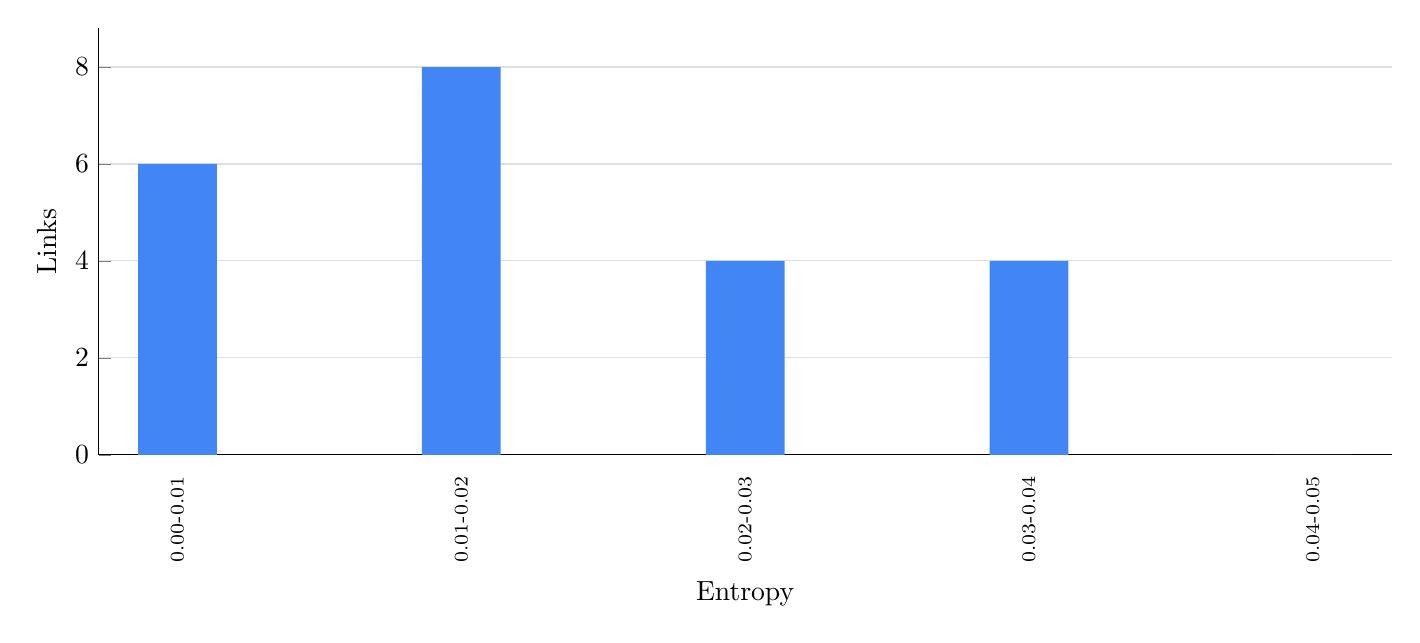
\begin{tikzpicture}
\begin{axis}[
  ybar, bar width=1.000cm, width=18.000cm, height=7cm,
  ymin=0, ymajorgrids, grid style={gray!25}, axis lines*=left,
  enlarge x limits={abs=1.000cm}, xtick=data, major x tick style={draw=none},
  x tick label style={rotate=90, font=\scriptsize, /pgf/number format/1000 sep=},
  legend style={at={(0.5,-0.3)}, anchor=north, legend columns=-1, draw=none},
  ylabel={Links},
  xlabel={Entropy},
  symbolic x coords={0.00-0.01,0.01-0.02,0.02-0.03,0.03-0.04,0.04-0.05,0.05-0.06,0.06-0.07,0.07-0.08,0.08-0.09,0.09-0.10,0.10-0.11,0.11-0.12,0.12-0.13,0.13-0.14,0.14-0.15,0.15-0.16,0.16-0.17,0.17-0.18,0.18-0.19,0.19-0.20,0.20-0.21,0.21-0.22,0.22-0.23,0.23-0.24,0.24-0.25,0.25-0.26,0.26-0.27,0.27-0.28,0.28-0.29,0.29-0.30,0.30-0.31,0.31-0.32,0.32-0.33,0.33-0.34,0.34-0.35,0.35-0.36,0.36-0.37,0.37-0.38,0.38-0.39,0.39-0.40,0.40-0.41,0.41-0.42,0.42-0.43,0.43-0.44,0.44-0.45,0.45-0.46,0.46-0.47,0.47-0.48,0.48-0.49,0.49-0.50,0.50-0.51,0.51-0.52,0.52-0.53,0.53-0.54,0.54-0.55,0.55-0.56,0.56-0.57,0.57-0.58,0.58-0.59,0.59-0.60,0.60-0.61,0.61-0.62,0.62-0.63,0.63-0.64,0.64-0.65,0.65-0.66,0.66-0.67,0.67-0.68,0.68-0.69,0.69-0.70,0.70-0.71,0.71-0.72,0.72-0.73,0.73-0.74,0.74-0.75,0.75-0.76,0.76-0.77,0.77-0.78,0.78-0.79,0.79-0.80,0.80-0.81,0.81-0.82,0.82-0.83,0.83-0.84,0.84-0.85,0.85-0.86,0.86-0.87,0.87-0.88,0.88-0.89,0.89-0.90,0.90-0.91,0.91-0.92,0.92-0.93,0.93-0.94,0.94-0.95,0.95-0.96,0.96-0.97,0.97-0.98,0.98-0.99,0.99-1.00}]
\addplot[fill={rgb,255:red,66;green,133;blue,244}, draw=none] coordinates {(0.00-0.01,6.000) (0.01-0.02,8.000) (0.02-0.03,4.000) (0.03-0.04,4.000) (0.04-0.05,0.000) };
\end{axis}
\end{tikzpicture}\end{center}
\clearpage
\section*{Shannon Entropy}
\begin{center}\begin{adjustbox}{max width=\linewidth}
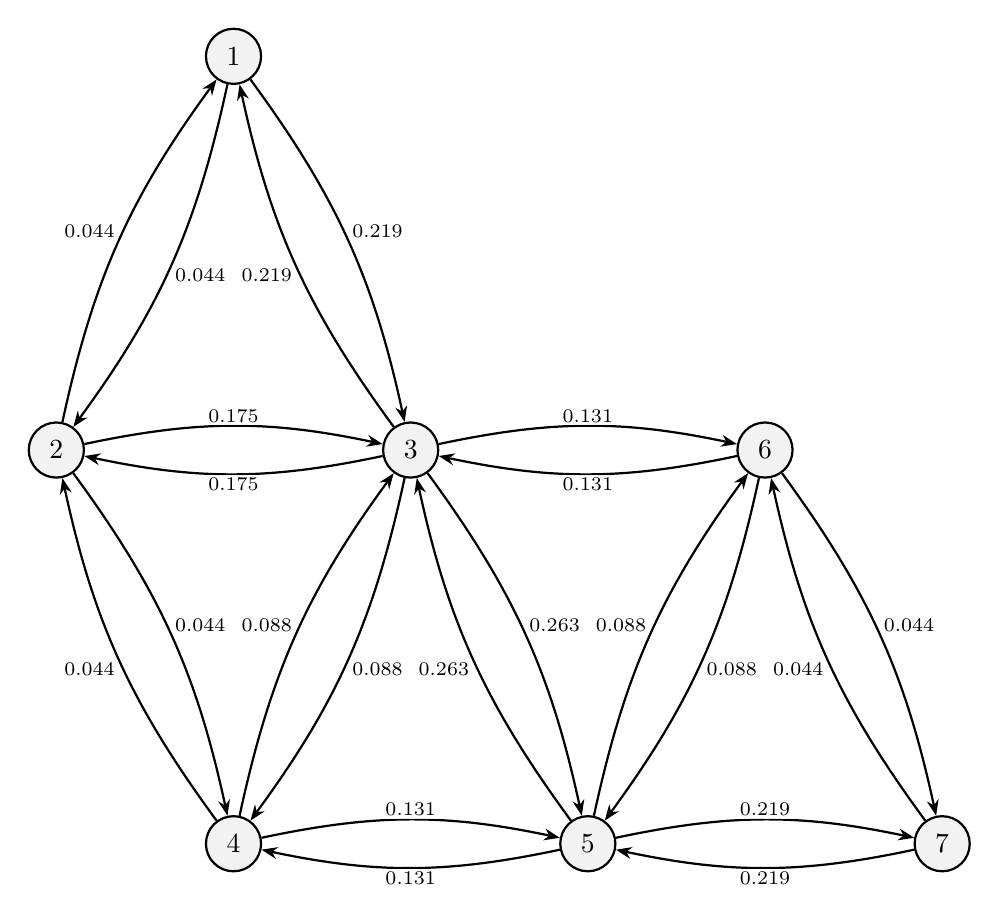
\begin{tikzpicture}[baseline, >={Stealth[length=2mm]},
  netnode/.style={circle, draw, thick, fill=gray!10, minimum size=7mm, inner sep=1pt},
  link/.style={thick},
  linklabel/.style={font=\scriptsize, inner sep=1pt, fill=white, fill opacity=0.85, text opacity=1}]
\node[netnode] (S1) at (2.250,10.000) {1};
\node[netnode] (S2) at (0.000,5.000) {2};
\node[netnode] (S3) at (4.500,5.000) {3};
\node[netnode] (S4) at (2.250,0.000) {4};
\node[netnode] (S5) at (6.750,0.000) {5};
\node[netnode] (S6) at (9.000,5.000) {6};
\node[netnode] (S7) at (11.250,0.000) {7};
\draw[link, ->] (S1) to[bend left=12] node[linklabel, auto] {0.044} (S2);
\draw[link, ->] (S1) to[bend left=12] node[linklabel, auto] {0.219} (S3);
\draw[link, ->] (S2) to[bend left=12] node[linklabel, auto] {0.044} (S1);
\draw[link, ->] (S2) to[bend left=12] node[linklabel, auto] {0.175} (S3);
\draw[link, ->] (S2) to[bend left=12] node[linklabel, auto] {0.044} (S4);
\draw[link, ->] (S3) to[bend left=12] node[linklabel, auto] {0.219} (S1);
\draw[link, ->] (S3) to[bend left=12] node[linklabel, auto] {0.175} (S2);
\draw[link, ->] (S3) to[bend left=12] node[linklabel, auto] {0.088} (S4);
\draw[link, ->] (S3) to[bend left=12] node[linklabel, auto] {0.263} (S5);
\draw[link, ->] (S3) to[bend left=12] node[linklabel, auto] {0.131} (S6);
\draw[link, ->] (S4) to[bend left=12] node[linklabel, auto] {0.044} (S2);
\draw[link, ->] (S4) to[bend left=12] node[linklabel, auto] {0.088} (S3);
\draw[link, ->] (S4) to[bend left=12] node[linklabel, auto] {0.131} (S5);
\draw[link, ->] (S5) to[bend left=12] node[linklabel, auto] {0.263} (S3);
\draw[link, ->] (S5) to[bend left=12] node[linklabel, auto] {0.131} (S4);
\draw[link, ->] (S5) to[bend left=12] node[linklabel, auto] {0.088} (S6);
\draw[link, ->] (S5) to[bend left=12] node[linklabel, auto] {0.219} (S7);
\draw[link, ->] (S6) to[bend left=12] node[linklabel, auto] {0.131} (S3);
\draw[link, ->] (S6) to[bend left=12] node[linklabel, auto] {0.088} (S5);
\draw[link, ->] (S6) to[bend left=12] node[linklabel, auto] {0.044} (S7);
\draw[link, ->] (S7) to[bend left=12] node[linklabel, auto] {0.219} (S5);
\draw[link, ->] (S7) to[bend left=12] node[linklabel, auto] {0.044} (S6);
\end{tikzpicture}
\end{adjustbox}\end{center}

\begin{center}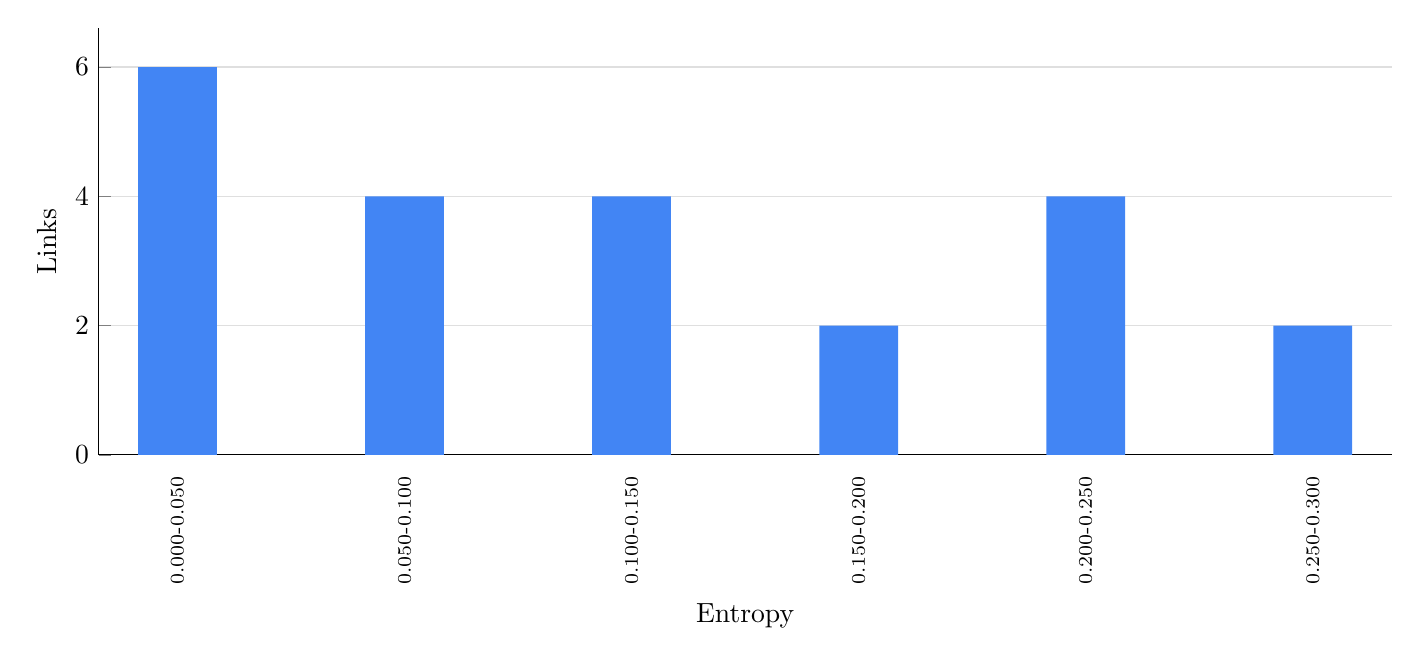
\begin{tikzpicture}
\begin{axis}[
  ybar, bar width=1.000cm, width=18.000cm, height=7cm,
  ymin=0, ymajorgrids, grid style={gray!25}, axis lines*=left,
  enlarge x limits={abs=1.000cm}, xtick=data, major x tick style={draw=none},
  x tick label style={rotate=90, font=\scriptsize, /pgf/number format/1000 sep=},
  legend style={at={(0.5,-0.3)}, anchor=north, legend columns=-1, draw=none},
  ylabel={Links},
  xlabel={Entropy},
  symbolic x coords={0.000-0.050,0.050-0.100,0.100-0.150,0.150-0.200,0.200-0.250,0.250-0.300,0.300-0.350,0.350-0.400,0.400-0.450,0.450-0.500,0.500-0.550,0.550-0.600,0.600-0.650,0.650-0.700,0.700-0.750,0.750-0.800,0.800-0.850,0.850-0.900,0.900-0.950,0.950-1.000}]
\addplot[fill={rgb,255:red,66;green,133;blue,244}, draw=none] coordinates {(0.000-0.050,6.000) (0.050-0.100,4.000) (0.100-0.150,4.000) (0.150-0.200,2.000) (0.200-0.250,4.000) (0.250-0.300,2.000) };
\end{axis}
\end{tikzpicture}\end{center}

\end{document}
